\documentclass{article}
\usepackage[utf8]{inputenc}
\usepackage{algorithmic}
\usepackage{algorithm}
\usepackage{amsmath,amsfonts,amssymb,amsthm}
\usepackage{mathtools}
\usepackage{commath}
\usepackage[sc,osf]{mathpazo}
\usepackage{algpseudocode}
\usepackage{pifont}
% \usepackage{amsmath}
\title{CS539 project: Verifying SVRG in practical nonconvex condition}
\author{Jui-Hung Lu }
\date{November 2019}

\usepackage{natbib}
\usepackage{graphicx}

\begin{document}

\maketitle
% \section{Abstract}
% S

\begin{abstract}
Stochastic gradient descent is a popular optimization, but there are lots of methods can improve the efficiency of SGD converging speed. Replicating the experiments from the paper by R. Johnson and T. Zhang [1], this paper implemented two different optimizers, SGD and SVRG, nonconvex condition. New data sets are used to verify whether the SVRG is useful with real-world data and situations.
\end{abstract}

\section{Introduction}
Stochastic gradient descent is the well-know optimizer in the machine learning area, but there are lots of issues that SGD. The trade-off between the speed of computation per iteration and convergence speed is one of the issues that SGD need to be solved. In R. Johnson and T. Zhang's paper, they point out that SGD needs a small learning rate is because of the variance of SGD. To solves this issue, they come up with a fixed SGD algorithm called stochastic variance reduced gradient (SVRG). SVRG used a snapshot weight and averaged a full gradient to control the weight updating at each time. Because the full gradient needs to be computed for a while, the memory cost needs to be a concern.
In this paper, we implemented a nonconvex condition by building a CNN model. With the CNN model, SDG and SVRG are included in training with real-world data which is the well-know dataset "Stanford Dog"[2]. In the end, there are two possible issues of SVRG that are found based on this experiment result.

\section{Problem Formulation and Algorithm}
In this paper, two algorithms are compared which are SGD and SVRG.
\subsection{SGD}
Based on the SGD pseudoㄦcode, SGD updating formulation shows below:
\[w^{(t)}=w^{(t-1)}-\eta_{t}\nabla\psi_{i_{t}}(w^{(t-1)}) \tag{1}\label{1}\]

In each iteration, SGD takes one randomly data to compute the loss function $\psi_{i_{t}}(w^{(t-1)})$ and weight updating. Lower memory is used in SGD than normal Gradient Descent. Therefore, in practical SGD has an advantage on large scale problem. However, each gradient $\nabla\psi_{i_{t}}(w^{(t-1)})$ is different, the variance is randomness. Thus, a constant learning rate of $\eta$ is used because of the variance of random data which causes the slow convergence.
\subsection{SVRG}
There is one of the methods to solve the SGD issue called stochastic variance reduced gradient (SVRG).
\begin{figure}[h!]
\centering
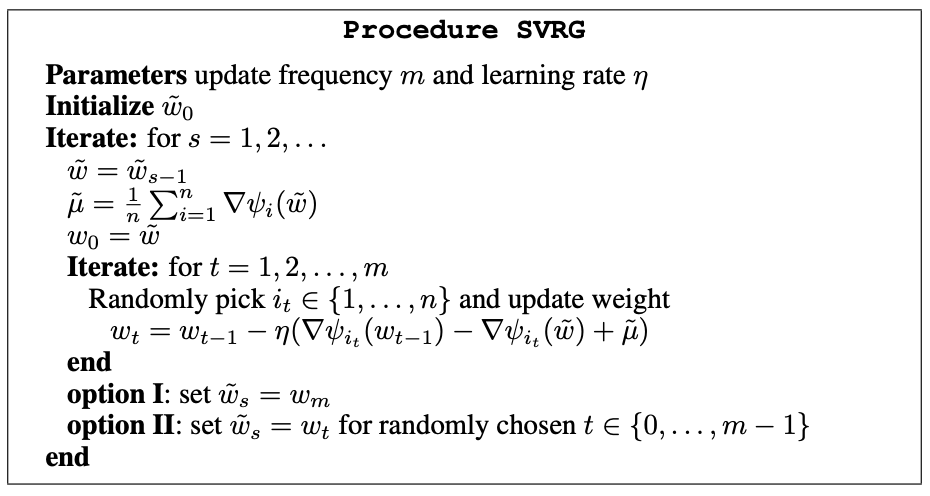
\includegraphics[scale=0.7]{SVRG.png}
\caption{Stochastic Variance Reduced Gradient [1] }
\label{fig:1}
\end{figure}

The summarized SVRG formulation from Figure \ref{fig:1}  shows below:
\[w^{(t)}=w^{(t-1)}-\eta_{t}(\nabla\psi_{i}(w^{(t-1)})-\nabla\psi_{i_{t}}\tilde{(w)}+\tilde{\mu})\tag{2}\label{2}\]
Each m iterations, SVRG keeps a snapshot of weight $\tilde{w}$ and computed the full gradient $\tilde{\mu}$. The variance is reduced by $\tilde{w}$ and $\tilde{\mu}$ that learning rate $\eta_{t}$ in SVRG does not need to decay.
% \subsection{Compare Formulation}
As we can see from \eqref{2}, in previous paper [1], it shows there is a bound that
\[\mathbf{E}[P\tilde{(w_{s})}-P(w_{*})]\leq \alpha^s\mathbf{E}[P\tilde{(w_{0})}-P(w_{*})]\]
,which it proves the SVRG converge condition.
\subsection{Compare Formulation}
As we see from SGD update\eqref{1}, we apply Dual Coordinate Ascent rule:
\[\alpha^{(t)}_{i}=\alpha^{(t-1)}_{i}-\eta_{t}(\nabla\phi_{i}(w^{(t-1)})+\lambda n\alpha^{(t-1)}_{i})
.\]
Because the convergence condition ($w_{*},\alpha_{*}$) we get
\[(\nabla\phi_{i}(w^{(t-1)})+\lambda n\alpha^{(t-1)}_{i})\xrightarrow{}0,
\]
the procedure can converge. In SVRG, it is similar as SGD:
\[\frac{1}{n}\sum_{i=1}^{n}(\nabla\phi_{i}(w^{(t-1)})+\lambda n\alpha^{(t-1)}_{i})^2 \xrightarrow{}0.
\]
Because of the square in SVRG, the variance goes to zero asymptotically and reduces the variance.
\section{Experiment}
To verify the theoretical result, the experiment compares the performance of SGD and SVRG with a convolutional neural network (nonconvex). In order to have more objective comparing results, the only difference is the optimizer.
\subsection{Environment}
About the experiment environment, all the calculation is working in Google Colaboratory for a highly stable cloud platform. CPU is used in this experiment. The Stanford Dog dataset[2] is applied to the experiment. In this dataset, there is 20580 number of images with 120 number of categories. Each image comes with three matrix data with size 224*224. The CNN model is built for training and testing using \emph{Pytorch}. The structure is showed in Table \ref{tab:1}, two convolution layers followed by batch normalization, Relu, 2*2 pool, and dropout to eliminate the noise of data. Then three linear layers reduce the dimension from 44944 to 120, which is the number of categories.
To setting the hyperparameters, we choose the learning rate 0.001 and batch size 32 that perform SGD best result. Because of the training time, the model is only trained with 2 epochs.
\newline
\begin{table}
\caption {CNN Structure} \label{tab:1} 
\begin{center}
\begin{tabular}{|l|c|c|c|c|c|}
\hline 
Layer&output&batchnorm&Relu&Pool&dropout\\
\hline  
conv2d_1&(6,110,110)&Yes&Yes&2*2&0.1\\
% \hline 
conv2d_2&(16,53,53)&Yes&Yes&2*2&0.1\\
% \hline 
flatten&(1,16*53*53)&&&&\\
% \hline 
linear_1&(1,120)&&Yes&&\\
% \hline 
linear_2&(1,84)&&Yes&&\\
% \hline 
linear_3&(1,120)&&&&\\
\hline 
\end{tabular}
\end{center}
\end{table}
\subsection{Optimizer}
The optimizer is the point in this experiment. We applied the library \emph{torch.optim} to built the comparing optimizer SGD. For SVRG, there are two ways to build the SVRG optimizer to make sure the correctness of this experiment. The first one is following the pseudo-code in Figure \ref{fig:1}, computer each necessary variable we need and calculus the weight updating directly. The second one, we built a custom optimizer by inherited the class \emph{Optimizer} in \emph{torch.optim}.

\subsection{Result}
First, we did the SVRG with the backward algorithm that we code completely without a library (Figure \ref{fig:2}).
Although the loss during training has no obvious difference, the reducing variance part $\tilde{w}$ and $\tilde{\mu}$ is work successful. Comparing with SGD, the loss decays smoothly and continuously. However, SGD converges with a better result after epoch 8.
\begin{figure}[h!]
\begin{subfigure}
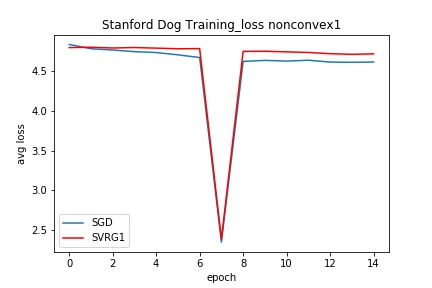
\includegraphics[width=.3\linewidth]{1_1.jpg}\hfill
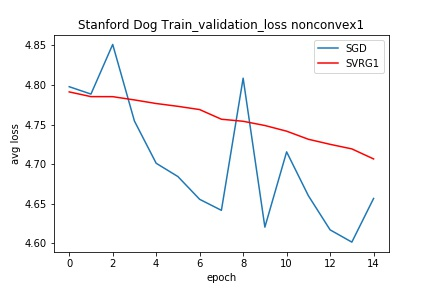
\includegraphics[width=.3\linewidth]{1_2.jpg}\hfill
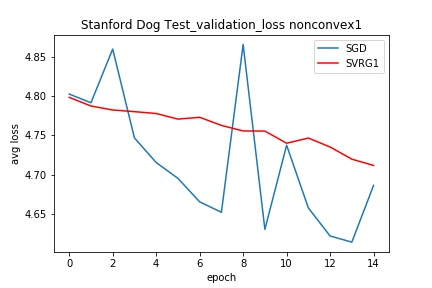
\includegraphics[width=.3\linewidth]{1_3.jpg}\hfill
\end{subfigure}
\caption{SVRG with pseudo code}
\label{fig:2}
\end{figure}
\begin{figure}[h!]
\begin{subfigure}
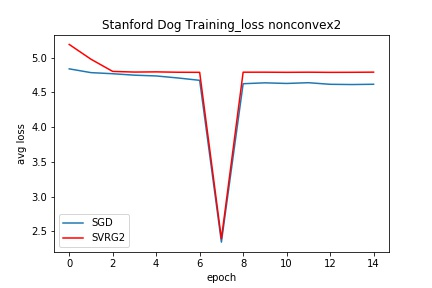
\includegraphics[width=.3\linewidth]{2_1.jpg}\hfill
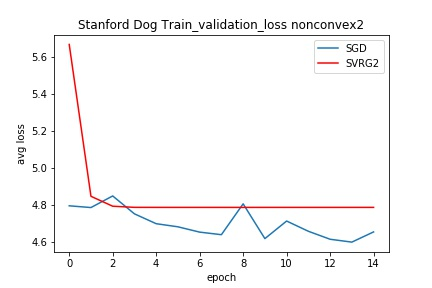
\includegraphics[width=.3\linewidth]{2_2.jpg}\hfill
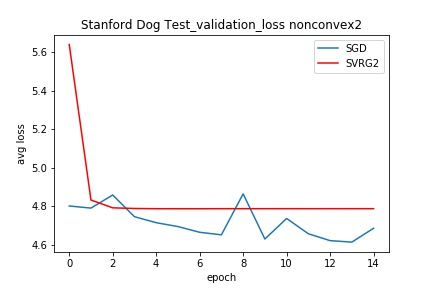
\includegraphics[width=.3\linewidth]{2_3.jpg}\hfill
\end{subfigure}
\caption{SVRG with custome torch optimizer}
\label{fig:3}
\end{figure}

Second, we implemented SVRG with a custom \emph{torch.optim} optimizer. The loss during training is the same as the previous method that has no obvious difference, but there is a large difference in the validation part. Although the validation error with SVRG decayed quickly and converged at epoch 2, the error in SGD didn't stop to decay. It might mean that this time our SVRG optimizer stick in a local minimum.

Taken the two building SVRG optimizer methods together, there are some issues can be
From all the results in both Figure \ref{fig:2} and Figure \ref{fig:3}, SVRG didn't have a better performance in our dataset. Although the reducing variance is obviously working, the convergence result of SVRG is not as expected as the result in R. Johnson and T. Zhang's paper. 
There are two possible reasons that the issue comes from. First, the gradient speed is reduced by too much noise. In practical, the dataset contains lots of unrelated information. Unlike the MNIST, there is no other information except the number in each photo. The reducing part of SVRG also reduces the model to remove the noise which also causes a higher error in the early epochs. We might adjust to a larger learning rate and seem if the issue can be solved.

Second, we think it may relate to the memory problem. In practical, the dataset is much complex and large than MNIST. The data from practical is not only larger but also triple time because of RGB images. Every time the SVRG did the full gradient, it not only cost much time but also much memory to calculate whole data loss. In order to control the memory problem, our CNN model can not contain too many layers. For example, the resnet101 has more than 40 layers of the entire network. The trade-off between memory control and accuracy causes the SVRG's performance in practice. 


\section{Conclusion}
This paper verified the variance reduction method for SVRG by comparing it with normal stochastic gradient descent in practical dataset Stanford-Dog. In non-convex condition, SVRG can still reduce variance and decay smoothly. However, SVRG has issues on slow convergence and sticks in a local minimum. It is not as expected as the result in small scale data like MNIST and CIFAR10 which is showing in the previous paper [1].
In this paper, we only set a constant learning rate in both SGD and SVRG. For the future experiment, large learning rate can be tested in SVRG since it provides the promise of reducing variance. Unlike SGD, a large learning rate can accelerate SVRG and may help SVRG get better performance in large-scale conditions.

\begin{thebibliography}{9}

\bibitem{accelerate_SGD} 
Rie Johnson and Tong Zhang. 
\textit 
Accelerating Stochastic Gradient Descent using Predictive Variance Reduction, 2013.

\bibitem{Stanford_Dog} 
Stanford Dogs Dataset. 
\textit 
http://vision.stanford.edu/aditya86/ImageNetDogs/.

\end{thebibliography}
\end{document}
